\documentclass[letterpaper, 12pt]{article}
\input{tex/_preamble}
\begin{document}
\flushleft\includegraphics[width=0.5\textwidth]{img/home/241017_final_logo_mockup.png}

\cosigsection{Data leakage}
\textit{Last updated: 2 July 2025}

Machine learning and other advanced statistical methods employ powerful algorithms that can fit too closely to one dataset but fail to generalize to new, unseen data. To mitigate against this, statisticians and modelers often split their data into a training set, on which the model is developed, and a test set, which is held back and later used to evaluated the model's performance. This approach gives a picture of how well the model might perform in practice on unseen data not available during training.

There are many variations on the training/test split approach. Datasets are commonly split 60:40 (such that 60\% of the available data is assigned to the training set and 40\% is assigned to the test set) or 70:30, but there is no universal rule-of-thumb. The goal is to maximize the amount of data available for training while holding back enough data to make a meaningful assessment of a model's performance. 

Another common approach, $k$-fold cross validation, involves partitioning a dataset into $k$ randomly-assigned ``folds'', holding out one of these folds as a test set and training on the remaining $k-1$ folds. The process is repeated for each of the $k$ folds, resulting in $k$ estimates of model performance. Often performed with 5 or 10 folds, this approach mitigates the impact of accidental class imbalances and ensures that each data point is used for validation exactly once. 

Yet another approach, Monte Carlo cross validation, randomly samples the dataset into a training set and test set without replacement, repeating training and evaluation over a given number of iterations. This approach gives more estimates of a given evaluation metric than a single training/test split or $k$-fold cross validation, but causes the same data points to be used in model evaluation multiple times.

Regardless of how a model is developed, one rule should never be broken: the test dataset must not in any way be contaminated with information from the training set (and vice versa). This contamination, often called ``data leakage'' or just ''leakage'', can lead to an overestimation of model performance. In practice there are many subtle ways that information can leak into the test set and bias model assessment. This guide covers some common types of data leakage.

\subsection*{Label leakage and illegitimate features}

Sometimes, features are included in a model's input that are either direct proxies for the outcome being predicted or are highly correlated with this outcome. For example, \href{https://ucsc-ospo.github.io/report/osre24/nyu/data-leakage/20240924-shaivimalik/}{consider a convolutional neural network trained to classify images as either depicting a husky or depicting a wolf}. While this model may appear to perform well when evaluated, this is only because the model has learned that images of huskies tend to have a green, grassy background and images of wolves tend to have a white, snowy background. In this case, the background of these images is an inappropriate feature that should be removed prior to model training. Models that prioritize inference from irrelevant features are often said to engage in \href{https://doi.org/10.1038/s42256-020-00257-z}{``shortcut learning''}.

%For instance, using a treatment assignment as a feature when predicting disease risk can lead to artificially high performance. This can happen even when researchers have good intentions, perhaps thinking that medication could be a confounder or covariate, and including it within the model. The problems with this can inherently be seen if a model is used to predict who might be at risk of hypertension, but the model includes whether the individuals took hypertensive medication. In one literature example , drugs such as losartan potassium featured in the model used to predict hypertension, but in fact are a consequence of the outcome. Another example might come from patient IDs from specific hospitals. A machine learning algorithm might learn that IDs from oncology hospitals have a higher risk of cancer, but this would be due to the patient already being admitted to an oncology hospital, not any form of risk.

\subsection*{Repeated measurements leakage}

In biological assays, individuals are often measured multiple times. These repeated measurements, known as technical replicates, should be averaged rather than treated as independent observations. Researchers may be tempted to treat technical replicates independently, as this superficially increases sample size and statistical power. However, these observations are not independent, and including them as such violates core assumptions of many statistical tests. This practice is often referred to a \href{https://en.wikipedia.org/wiki/Pseudoreplication}{``pseudoreplication''}.

Worse, if one replicate (e.g., ``Sam One'') is in the training set and another from the same source (e.g., ``Sam Two'') is in the test set, the model gains an unfair advantage; it has effectively already ``seen'' this element of the test data since the two replicates are highly similar. This can also occur when data are inadvertently duplicated (e.g., ``Sam One'' is in both the training and test sets).

\begin{figure}[h!tbp]
    \centering
    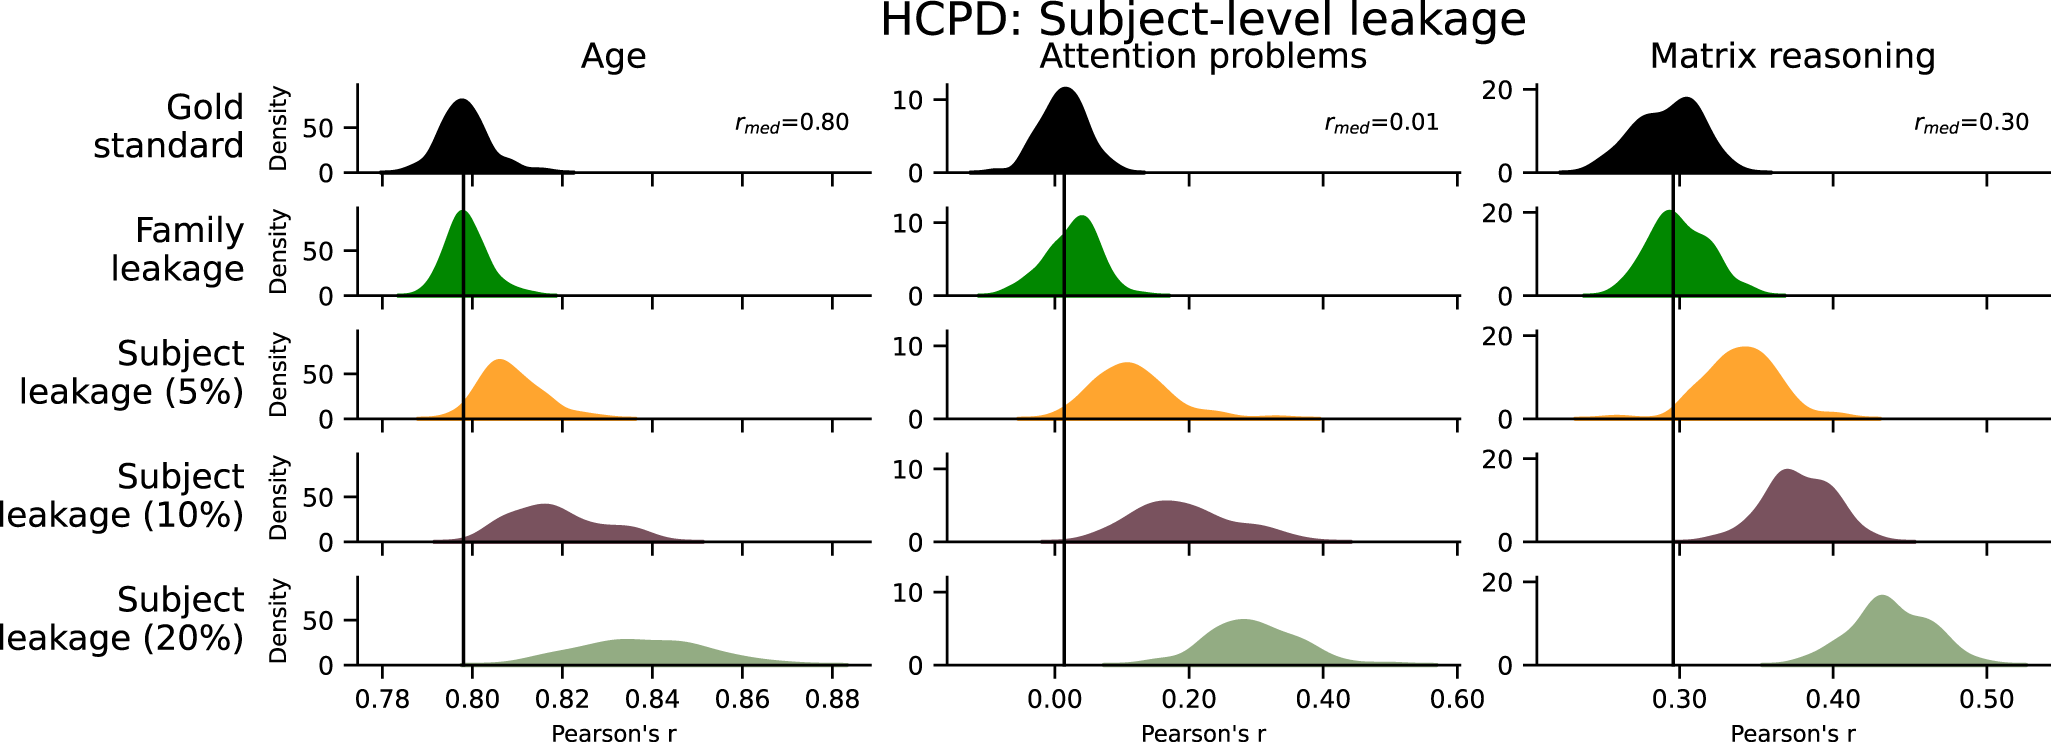
\includegraphics[width=\textwidth]{img/leakage/rosenblatt_fig_5.png}
    \caption*{\href{https://doi.org/10.1038/s41467-024-46150-w}{Rosenblatt et al. (2024)} describe how data leakage can inflate the predictive performance of models trained on functional magnetic resonance imaging (fMRI) data. For the figure above, they demonstrate how performance (measured by Pearson's r) for predicting a subject's age, attention problems and reasoning skills increases when family members of subjects in the training set are included in the test set (``family leakage'') and when a certain percentage of subjects in the entire dataset are duplicated (``subject leakage'').}
\end{figure}

\subsection*{Feature selection leakage}

Feature selection is a critical step in building predictive models. However, it can become a major source of data leakage  if not done properly. Leakage occurs when features are selected using the entire dataset including the test set. For example, selecting features based on correlation with the outcome variable using the full dataset introduces bias; the model appears to perform better because it has been indirectly exposed to the test data.

To prevent this, feature selection should always be performed after the train-test split and only on the training data. Evaluations such as correlation, mutual information or feature importance scores must be restricted to the training portion. In cross-validation or nested cross-validation, feature selection must occur within each fold of the training data to avoid leakage across folds.

\subsection*{Leakage due to data pre-processing}

Data leakage can also occur during pre-processing steps such as normalization, imputation, or scaling, if these are performed using the full dataset. For instance, if the mean and standard deviation used to scale a feature are computed using both training and test data, the model benefits from knowledge of the test set. This undermines the goal of a fair evaluation. To avoid this, all pre-processing steps must be fitted using only the training data and then applied to the test set.

\subsection*{Temporal leakage}

In time series or longitudinal datasets, using future information to predict the past introduces temporal leakage. A model that includes information not available at the time of prediction will perform unrealistically well in validation but poorly in practice. Proper chronological splitting is critical: the training data must come entirely from earlier time points than the test data.

\subsection*{Leakage due to bias in study design}

There is one final, subtle form of data leakage that is harder to eliminate: systematic bias in study design. A single study will often recruit participants using specific criteria, locations or instruments. As a result, the people in the test dataset are often more similar to those in the training dataset than would be expected in a truly random population sample. This gives the model an unintended advantage since it is being tested on data that closely resembles the training data.

This issue can also be caused by differences in instrumentation. For instance, if a particular instrument is particularly good at detecting certain features, this benefit applies equally to both training and test sets. But in a broader population or with a different instrument, the performance may degrade. 

This highlights a fundamental limitation of single-study validation: even when a dataset is perfectly split and free from leakage in the traditional sense, true generalizability can only be assessed using an independent dataset, ideally from a different cohort, with different equipment, analyzed in a separate laboratory.

\subsection*{Recognizing data leakage}

Data leakage can be difficult to recognize without a detailed understanding of how datasets were handled for model training and evaluation. Thus, it is critical that articles report precisely which features were used during model training, how training/test splits were performed and how model performance was evaluated. In the absence of this information, common warning signs that data leakage has occurred include a model performing markedly better for the test set than for the training set and unrealistically high model performance (e.g., a model successfully predicting  an autism diagnosis with no false positives and no false negatives).

\subsection*{Example 1: Label leakage}

\href{https://doi.org/10.2196/jmir.9268}{Ye et al. (2018)} describe applying machine learning to patient electronic health records (EHRs) to build a model capable of predicting incident hypertension within the next year. They report that their model has excellent predictive performance: an area under the \href{https://en.wikipedia.org/wiki/Receiver_operating_characteristic}{receiver operating characteristic} curve (AUROC) of 0.870. However, as noted by \href{https://doi.org/10.2196/10969}{Filho et al. (2021)}, the authors include 98 medication prescriptions as input variables, including several drugs popularly used to treat hypertension. Five of these antihypertensive drugs are among the six most influential features of the model for predicting hypertension (as measured by odds ratio). These features are a consequence of the outcome being predicted (patients are prescribed antihypertensive drugs because they have hypertension) and not the other way around (patients do not develop hypertension because they are prescribed antihypertensive drugs). Thus, the inclusion of these features causes data leakage and likely inflates the model's predictive performance.

\subsection*{Example 2: Feature selection leakage}

\href{https://doi.org/10.1186/s12887-016-0586-x}{Hicks et al. (2016)} profile microRNAs in saliva of children with autism spectrum disorder (ASD) and matched controls (45 subjects in total). Of 246 microRNAs included in the following analysis, the authors select 14 microRNAs that are differentially expressed between the ASD and control groups and use these features to construct a multivariate logistic regression that they claim is capable of distinguishing ASD from non-ASD with high accuracy. Although the authors perform Monte Carlo cross-validation, the 14 features underlying the models they train were selected from the full dataset without any subjects held out as a test group. Thus, this model was developed using the same dataset it is later evaluated over. As noted by \href{https://pubpeer.com/publications/474BE49866A9B1F37690E6FDA5C104}{Marantochloa filipes on PubPeer}, this same procedure will result in high predictive performance even when the underlying data is generated so that there are no actual differences between the control and ASD groups.

\subsection*{Example 3: Temporal leakage}

\href{https://doi.org/10.1109/ICSE.2012.6227210}{Zhou et al. (2012)} describe a procedure for automatically identifying the location of bugs in code based off of the summary of the initial bug report. However, as detailed by \href{https://doi.org/10.1145/3236024.3236054}{Tu et al. (2018)}, the dataset used by Zhou et al. includes the summary of bug reports at the time of data retrieval, not at the time the bug reports were initially filed. Many of the bug reports submitted were modified, which may have occurred after developers already identified the bug's location. This information would not be available when the model is deployed on actual new bug reports in real time. Tu et al. demonstrate that using each bug report's initial summary instead of its modified summary decreases model performance. Thus, part of the model's high performance is attributable to temporal data leakage.

\subsection*{Example 4: Illegitimate features}

\href{https://doi.org/10.3233/XST-200715}{Rahaman et al. (2020)} report on using pre-trained convolutional neural networks to distinguish between chest X-ray images from COVID-19 patients, non-COVID-19 pneumonia patients and normal cases with high accuracy. However, as noted by \href{https://doi.org/10.1038/s42256-021-00307-0}{Roberts et al. (2021)}, the COVID-19 chest X-rays used are all from adult patients and the non-COVID-19 pneumonia and normal chest X-rays are all from pediatric patients. Thus, the models tested can discriminate between COVID-19 and non-COVID-19 cases simply by detecting which X-rays depict children and which depict adults using features that are not clinically relevant. In fact, as demonstrated by \href{https://doi.org/10.1016/j.inffus.2021.04.008}{Maguolo and Nanni (2021)}, a convolutional neural network can be trained to distinguish these datasets from eachother with high performance even when the region depicting the lungs is edited out of every image. \href{https://ucsc-ospo.github.io/report/osre24/nyu/data-leakage/20240924-shaivimalik/}{Malik (2024)} demonstrates that performance on this task drops markedly when datasets containing only adult patients are used.

\subsection*{Example 5: Leakage during training, leakage due to study design}

\href{https://arxiv.org/abs/2306.08997v1}{Zhang et al. (2023)} report on using the large language models GPT-3.5 and GPT-4 to answer questions from the Massachusetts Institute of Technology (MIT) engineering curricula. Their preprint asserts the \href{https://www.chronicle.com/newsletter/weekly-briefing/2023-07-15}{widely-publicized} claim that ChatGPT could earn an engineering degree from MIT. However, as demonstrated by \href{https://flower-nutria-41d.notion.site/No-GPT4-can-t-ace-MIT-b27e6796ab5a48368127a98216c76864}{Chowdhury et al. (2023)}, the \href{https://en.wikipedia.org/wiki/Few-shot_learning}{few-shot learning approach} used by the authors effectively prompted these models with incredibly similar versions of the questions that they would subsequently be tested on. Moreover, for some questions, the model was effectively prompted until the correct answer was achieved. Thus, at evaluation, the model had access to information it should not have: whether its own initial answers were correct.

The preprint by Zhang et al. was \href{https://doi.org/10.48550/arXiv.2306.08997}{withdrawn} shortly after Chowdhury et al. published their initial review.

\subsection*{Additional resources}

\begin{itemize}
    \setlength\itemsep{-0.5em}
     \item \href{https://doi.org/10.1016/j.patter.2023.100804}{``Leakage and the reproducibility crisis in machine-learning-based science'' (2023)}
     \item \href{https://doi.org/10.1038/s42256-020-00257-z}{``Shortcut learning in deep neural networks'' (2020)}
     \item \href{https://doi.org/10.1038/s41592-024-02362-y}{``Guiding questions to avoid data leakage in biological machine learning applications'' (2024)}
     \item \href{https://doi.org/10.1117/12.2549313}{``Hazards of data leakage in machine learning: a study on classification of breast cancer using deep neural networks'' (2020)}
     \item \href{https://doi.org/10.1038/s41467-024-46150-w}{``Data leakage inflates prediction performance in connectome-based machine learning models'' (2024)}
     \item \href{https://doi.org/10.1145/3236024.3236054}{``Be careful of when: an empirical study on time-related misuse of issue tracking data'' (2018)}
     \item \href{https://www.ibm.com/think/topics/data-leakage-machine-learning}{``What is data leakage in machine learning?''}
\end{itemize}

\end{document}